% =============================================================================
% CalibPL: Dual Isotonic Calibration Reveals the Hidden Failure Mode of
%          Semi-Supervised Detection in Dense Scenes
%
% WACV 2027 Submission  |  Algorithms Track
% Double-blind anonymized -- do NOT include author names or affiliations.
% =============================================================================

\documentclass[10pt,twocolumn,letterpaper]{article}
\usepackage{wacv}   % WACV 2027 style

%% ---- Essential packages ----------------------------------------------------
\usepackage{amsmath,amssymb,amsfonts,amsthm}
\usepackage{algorithm}
\usepackage{algpseudocode}
\usepackage{booktabs}
\usepackage{enumitem}
\usepackage{xcolor}
\usepackage{graphicx}
\usepackage{multirow}
\usepackage{microtype}  % better paragraph shaping; prevents overfull hboxes
\usepackage{url}
\usepackage{xspace}
\usepackage{pifont}         % for \ding{51} checkmark / \ding{55} cross in tables

%% ---- Theorem environments --------------------------------------------------
\newtheorem{proposition}{Proposition}
\newtheorem{corollary}{Corollary}
\newtheorem{definition}{Definition}
\newtheorem{lemma}{Lemma}
\newtheorem{theorem}{Theorem}

%% ---- Paper-specific macros -------------------------------------------------
\newcommand{\method}{\textbf{CalibPL}\xspace}
\newcommand{\coco}{\textsc{COCO}\xspace}
\newcommand{\sku}{\textsc{SKU-110K}\xspace}
\newcommand{\deltaece}{\Delta\!\operatorname{ECE}}

%% ============================================================================
\begin{document}
%% ============================================================================

%% ---------------------------------------------------------------------------
%%  TITLE + ABSTRACT: use \twocolumn[...] so both span the full page width.
%%  This is the standard CVF idiom (used by CVPR/ICCV/WACV official templates).
%% ---------------------------------------------------------------------------
\twocolumn[{%
\begin{center}
  {\LARGE\bfseries CalibPL: Dual Isotonic Calibration Reveals the Hidden\\
   Failure Mode of Semi-Supervised Detection in Dense Scenes}\par
  \vspace{0.5em}
  {\large Anonymous Author(s)\\
  {\normalsize\ttfamily anonymous@institution.edu}}\par
  \vspace{0.3em}
\end{center}
\vspace{0.4em}
\noindent\rule{\linewidth}{0.2pt}\vspace{0.2em}

% ============================================================================
\begin{wacvabstract}
% ============================================================================
Semi-supervised object detection (SSOD) assumes that classification confidence
reliably proxies pseudo-label spatial quality. We prove---mathematically and
empirically---that this assumption \emph{collapses} in dense scenes through a
mechanism we call the \textbf{NMS Tail Amplification} effect. Non-Maximum
Suppression selects the highest-classification-score survivor from each dense
cluster; localization quality is a passenger, not selected for. We formalize
this as Proposition~\ref{prop:nms_tail} and show that the expected gap between
classification confidence and localization accuracy grows \emph{monotonically}
with NMS competition size~$n$. Consequently, Consistent-Teacher's GMM
thresholding \emph{doubles} localization ECE from 0.113 to 0.226 on \sku\
($\bar{\rho}{\approx}147$~obj/img), producing pseudo-labels where
\textbf{39\% of high-confidence boxes have IoU$<$0.5}. Crucially, \emph{static}
post-hoc calibration---which achieves strong results on fixed supervised
detectors~\cite{kuzucu2024calibration}---fails under iterative SSOD because the
score distribution shifts at each pseudo-label generation cycle; a
once-fitted calibrator accrues 0.024 ECE drift by iteration~1.
To address this, we propose \method, which fits \emph{dual isotonic
calibrators}---one for classification, one for localization---\emph{re-fitted
at every iteration} to track distribution shift, combined with a
Class-Geometry Joint Stability (CGJS) gate requiring both spatial and semantic
consistency under augmentation.
\method\ improves pseudo-label precision by \textbf{+23~pp} ($0.61{\to}0.84$),
reduces false positives by \textbf{$\sim$70\%}, and achieves
\textbf{88.48$\pm$0.11~AP$_{50}$} on dense retail scenes---a \textbf{+1.20
AP$_{50}$ improvement over our strongest in-protocol baseline} (Fixed
$\tau{=}0.5$, identical recipe, seeds, and architecture). The theory makes a
falsifiable prediction---no AP gain on sparse \coco\ ($\rho {<} \kappa$)---which
experiments confirm precisely ($p{=}0.41$). Cross-domain validation on
CrowdHuman demonstrates +8.3~AP over 3~self-training iterations, confirming
density-driven generalization.
\end{wacvabstract}
\vspace{0.3em}
\noindent\rule{\linewidth}{0.2pt}
\vspace{0.8em}
}] % end \twocolumn[...]

% ============================================================================
\section{Introduction}
\label{sec:intro}
% ============================================================================

\begin{figure*}[!t]
  \centering
  \includegraphics[width=0.92\textwidth]{../../results/figures/ece_drift_fig1_wide.png}
  \vspace{-4pt}
  \caption{\textbf{The hidden failure mode of dense SSOD.} ECE drift across
  5 self-training iterations.
  \textit{Left}: Sparse \coco ($\bar{\rho}{\approx}7$): mild divergence.
  \textit{Right}: Dense \sku ($\bar{\rho}{\approx}147$): localization ECE
  \emph{explodes} while classification ECE stays bounded (shaded
  ``dual misalignment zone''). A static post-hoc calibrator, applied once
  after training, cannot track this drift.}
  \label{fig:ece_drift}
  \vspace{-6pt}
\end{figure*}

Every state-of-the-art semi-supervised object detector makes the same silent
assumption: that a detector's classification confidence can proxy pseudo-label
spatial quality. The teacher-student self-training
paradigm~\cite{unbiasedteacher2021,softteacher2021,consistentteacher2023},
currently the dominant approach to SSOD, is built entirely on this assumption.
On sparse benchmarks like \coco ($\bar{\rho}{\approx}7$~obj/img), this
is adequate. Dense scenes expose a qualitatively different, previously
uncharacterized failure mode.

\textbf{The failure mode.}
On \sku~\cite{sku110k2019} ($\bar{\rho}{=}141.95{\pm}32.4$~obj/img),
Consistent-Teacher's~\cite{consistentteacher2023} GMM-based adaptive
thresholding \emph{doubles} localization ECE from 0.113 to 0.226,
measured on $n{=}16{,}393$ detection samples (Figure~\ref{fig:ece_drift}).
\textbf{39\% of pseudo-boxes accepted at $\hat{p}_\text{cls}{\ge}0.5$ have IoU~$<$~0.5} (measured across all confidence bins above the threshold; the high-score tail alone has 26--28\% mis-localization rate, see Table~A.1 in Supplementary~A).
The student trains on pseudo-labels that \emph{look confident but are spatially
unreliable}, and this error compounds across self-training iterations.

\textbf{Why static post-hoc calibration fails here.}
Recent work~\cite{kuzucu2024calibration} has shown that post-hoc calibration
methods---particularly Platt Scaling and Isotonic Regression---outperform
complex training-time calibration methods for object detectors in the
fully-supervised, fixed-model setting. However, in iterative SSOD, the model
evolves at every pseudo-label generation cycle, causing the score distribution
to shift. A calibrator fitted at iteration~0 accrues ECE drift of 0.024 by
iteration~1 (Table~\ref{tab:adaptive_vs_static}). We prove formally
(Proposition~\ref{prop:nms_tail}) that this drift is a
\emph{structural consequence} of NMS dynamics in dense scenes, not a tuning
artifact. The setting of Kuzucu et al.~\cite{kuzucu2024calibration} is
fundamentally different: a static, fully-supervised model at inference time,
where no distribution shift occurs. Their strong results do not transfer to
iterative SSOD.

\textbf{Our solution.}
\method\ replaces the single confidence proxy with \emph{two independent
isotonic calibrators}: one mapping classification confidence to
$\Pr(\text{cls~correct})$, and one mapping the CGJS stability score $\sigma_b$
(augmentation consistency fraction, Eq.~\ref{eq:cgjs}) to
$\Pr(\text{IoU}{\ge}0.5)$. Both are \emph{re-fitted at each self-training
iteration} via stratified bootstrap, maintaining near-perfect calibration
(ECE~${<}0.003$) throughout the entire training process. The CGJS gate
further filters predictions that are unstable under augmentation. Together, they achieve $+23$~pp pseudo-label
precision and $+1.20$~AP$_{50}$ over our in-protocol Fixed~$\tau{=}0.5$
baseline on dense retail scenes, while theoretically predicting (and
empirically confirming) zero AP gain on sparse \coco.

\paragraph{Contributions.}
\begin{itemize}[noitemsep,topsep=2pt,leftmargin=*]
  \item \textbf{NMS Tail Amplification Proposition}: formal proof that NMS
    decouples classification and localization calibration in proportion to
    competition size, with density onset at $\kappa{\approx}12$~obj/img.
  \item \textbf{Dynamic Dual Isotonic Calibration}: per-iteration,
    distribution-free, stratified-bootstrap pseudo-label quality estimator
    that tracks score distribution shift---the key mechanism missing in static
    post-hoc approaches~\cite{kuzucu2024calibration}---achieving
    held-out ECE~${<}0.003$ vs.\ 0.226 for GMM (Table~\ref{tab:calibration}).
  \item \textbf{CGJS gate}: lightweight stability filter requiring joint
    spatial and semantic consistency, catching semantically-confused
    predictions missed by geometry-only methods~\cite{pseco2022}.
  \item \textbf{Falsifiable prediction and confirmation}: CalibPL
    predicts \emph{no} AP gain on sparse \coco\ ($\rho{<}\kappa$);
    experiments confirm this ($p{=}0.41$, two-tailed $t$-test).
  \item \textbf{Cross-domain validation}: on CrowdHuman
    ($\bar{\rho}{\approx}22$), CalibPL prevents AP collapse and delivers
    +8.3~AP by iteration~3.
\end{itemize}

% ============================================================================
\section{Related Work}
\label{sec:related}
% ============================================================================

\paragraph{Semi-supervised object detection.}
STAC~\cite{stac2020}, Unbiased Teacher~\cite{unbiasedteacher2021},
Soft Teacher~\cite{softteacher2021}, Dense
Teacher~\cite{denseteacher2022}, Consistent-Teacher~\cite{consistentteacher2023},
EfficientTeacher~\cite{efficientteacher2023}, and
SoftMatch~\cite{softmatch2023} all use a single confidence score or GMM as a
universal quality proxy. PseCo~\cite{pseco2022} adds geometric consistency but
not calibration. \emph{None} separates classification from localization
calibration, which is the critical gap we address (Table~\ref{tab:taxonomy}).
Recent WACV works on semi-supervised learning in dense
domains~\cite{mvat2026,reflectiveteacher2025} focus on 3D/BEV detection with
uncertainty but do not address the iterative calibration drift problem in 2D
dense scenes.

\begin{table}[t]
  \centering
  \caption{\textbf{SSOD filtering taxonomy.} \method\ uniquely provides
  separate non-parametric calibration for both quality axes, per-iteration
  re-fitting to track distribution shift, and dense-scene support.}
  \vspace{2pt}
  \setlength{\tabcolsep}{3pt}
  \resizebox{\columnwidth}{!}{%
  \begin{tabular}{lccccc}
    \toprule
    Method & Cls Cal. & Loc Cal. & Dynamic & Stability & Dense \\
    \midrule
    STAC~\cite{stac2020}                        & Fixed & --  & --  & --      & \ding{55} \\
    Soft Teacher~\cite{softteacher2021}          & Fixed & Jit & --  & --      & \ding{55} \\
    Unbiased Teacher~\cite{unbiasedteacher2021}  & Fixed & --  & --  & Weak    & \ding{55} \\
    PseCo~\cite{pseco2022}                       & Fixed & --  & --  & Geo.    & \ding{55} \\
    CT~\cite{consistentteacher2023}              & GMM   & --  & --  & --      & Degrades  \\
    Kuzucu \etal~\cite{kuzucu2024calibration}    & Iso.  & --  & \ding{55} & -- & \ding{55} \\
    \textbf{CalibPL (Ours)} & \textbf{Iso.} & \textbf{Iso.} & \textbf{\ding{51}} & \textbf{Cls+Geo} & \textbf{\ding{51}} \\
    \bottomrule
  \end{tabular}}
  \label{tab:taxonomy}
  \vspace{-6pt}
\end{table}

\paragraph{Calibration in object detection.}
Guo~\etal~\cite{guo2017calibration} established calibration theory for
classification. K\"{u}ppers~\etal~\cite{kuppers2020detector} extended this to
Detection ECE (D-ECE). Jiang~\etal~\cite{iounet2018} (ECCV 2018) introduced
IoU-Net, which predicts localization quality (IoU) as a separate branch
and uses it to re-rank NMS survivors---directly addressing the cls/loc
decoupling in the supervised, fixed-model setting. \method\ differs fundamentally:
IoU-Net modifies NMS at inference to improve final detections, while \method\
operates during iterative self-training pseudo-label generation where score
distributions shift each iteration. The most closely related work is
Kuzucu~\etal~\cite{kuzucu2024calibration} (ECCV 2024), who demonstrate that
post-hoc Platt Scaling and Isotonic Regression outperform training-time
calibration on COCO in the \emph{fully-supervised, fixed-model} setting.
Table~\ref{tab:kuzucu_diff} makes the mechanistic difference explicit: their
setting involves a \emph{static} model at inference time (no distribution
shift), while our SSOD setting has an \emph{evolving} teacher that induces
distribution shift at every iteration. Our contribution is complementary and
distinct in three ways: (1)~we target the \emph{iterative SSOD} regime
requiring dynamic per-iteration re-fitting; (2)~we calibrate both
classification \emph{and} localization jointly; (3)~we provide Proposition~1
explaining why any static post-hoc calibrator accrues drift under NMS dynamics.
Applying the static isotonic variant (as in~\cite{kuzucu2024calibration})
to our pipeline achieves intermediate improvement but leaves significant drift
by iteration~3 (ECE$_\text{loc}$: 0.021 vs.\ our $\approx$0).

\begin{table}[t]
  \centering
  \caption{\textbf{CalibPL vs.\ Kuzucu \etal~\cite{kuzucu2024calibration}:
mechanistic comparison.} The two works are \emph{complementary}---not
competing---because the settings differ fundamentally.}
  \vspace{2pt}
  \setlength{\tabcolsep}{4pt}
  \resizebox{\columnwidth}{!}{%
  \begin{tabular}{lcc}
    \toprule
    \textbf{Aspect} & \textbf{Kuzucu \etal~\cite{kuzucu2024calibration}} & \textbf{CalibPL (Ours)} \\
    \midrule
    Setting         & Supervised, fixed model & Iterative SSOD, evolving teacher \\
    Distribution shift & None at inference & Every iteration \\
    Calibration timing & Post-hoc, \emph{once} & Per-iteration, \emph{dynamic} \\
    Axes calibrated & Classification only & Cls \emph{and} localization \\
    Dense scenes    & Not studied & Core contribution \\
    Formal theory   & Empirical only & Proposition~1 (NMS Tail Amplif.) \\
    \bottomrule
  \end{tabular}}
  \label{tab:kuzucu_diff}
  \vspace{-6pt}
\end{table}

Popordanoska~\etal~\cite{popordanoska2024} (WACV 2024) provide a density-based
calibration estimator for detection but focus on measurement, not solution, and
do not address the SSOD training loop.
Porcher~\etal~\cite{metacalib2025} apply temperature scaling to pseudo-labels
for instance segmentation but use a static single-pass calibrator.

\paragraph{Dense detection.}
Dense-scene papers~\cite{sku110k2019,crowdhuman2018,visdrone2018,densessod2021}
focus on architectural improvements (density-aware NMS, relation modules). We
show dense scenes are fundamentally a \emph{calibration drift} problem under
semi-supervised training. Isotonic regression~\cite{ayer1955empirical,robertson1988order}
was applied to classification calibration~\cite{zadrozny2002} but not, to our
knowledge, to \emph{localization} calibration inside iterative SSOD loops.

% ============================================================================
\section{Method}
\label{sec:method}
% ============================================================================

\begin{figure}[!t]
  \centering
  \includegraphics[width=0.90\columnwidth]{../../results/figures/figure2_architecture.png}
  \vspace{-2pt}
  \caption{\textbf{The CalibPL pipeline.} Boxes from $f_t$ are independently
  calibrated for classification ($g_t^\text{cls}$, blue) and localization
  ($g_t^\text{loc}$, green), re-fitted at every iteration. The CGJS gate
  (yellow) requires both spatial IoU and class-agreement consistency under
  augmentation. Only pseudo-labels passing all three gates train $f_{t+1}$.}
  \label{fig:architecture}
  \vspace{-8pt}
\end{figure}

\subsection{Problem Setup}

Let $\mathbf{D}_L{=}\{(x_i,y_i)\}_{i=1}^{N_L}$ be labeled images and
$\mathbf{D}_U{=}\{u_j\}_{j=1}^{N_U}$ unlabeled images. At iteration~$t$,
detector $f_t$ produces candidate boxes $b$ with classification score
$\hat{p}_\text{cls}(b)$ and CGJS stability score $\sigma_b(b)$ (Eq.~\ref{eq:cgjs}). We
select pseudo-labeled set $\widetilde{\mathbf{D}}_U^{(t)}$ to train $f_{t+1}$
(Figure~\ref{fig:architecture}).

\subsection{NMS Tail Amplification}
\label{sec:dual_misalignment}

\begin{definition}[NMS Survivor]
Given $n$ candidates $\{(S_i,L_i)\}_{i=1}^n$ where $S_i{\in}[0,1]$ is
classification score and $L_i{=}\mathbf{1}[\text{IoU}{\ge}0.5]$ localization
correctness, NMS selects $I^*{=}\arg\max_i S_i$, yielding survivor $(S^*,L^*)$.
\end{definition}

\begin{proposition}[NMS Tail Amplification]
\label{prop:nms_tail}
Let $g(s){:=}\Pr(L{=}1\mid S{=}s)$ be the true precision-at-confidence
function. Suppose $g(s){\le}s{-}\delta$ for all $s{\ge}s_0$ \emph{(tail
overconfidence)}. Then the expected overconfidence of the NMS survivor satisfies:
\[
\Delta_n := \mathbb{E}[S^*] - \mathbb{E}[g(S^*)] \;\ge\; \delta\bigl(1-F_S(s_0)^n\bigr),
\]
where $F_S$ is the CDF of $S$. The bound is \emph{strictly increasing} in
competition size $n$ whenever $F_S(s_0){\in}(0,1)$.
\end{proposition}

\begin{proof}[Proof sketch]
NMS selects $S^*{=}\max_i S_i$, so by order statistics
$\Pr(S^*{\ge}s_0){=}1{-}F_S(s_0)^n\to1$ as $n\to\infty$.
Applying the tail overconfidence bound to the conditional expectation and
integrating over $[s_0,1]$ yields $\Delta_n \ge \delta\cdot\Pr(S^*{\ge}s_0)$.
Full proof with technical conditions in Supplementary~A.
\end{proof}

\begin{corollary}[Density-Dependence]
\label{cor:density}
Scene density $\rho$ drives NMS competition size $n$.
Below $\kappa$, $\Delta_n{\approx}0$; above $\kappa$, $\Delta_n{>}\delta/2$.
\end{corollary}

\begin{figure}[!t]
  \centering
  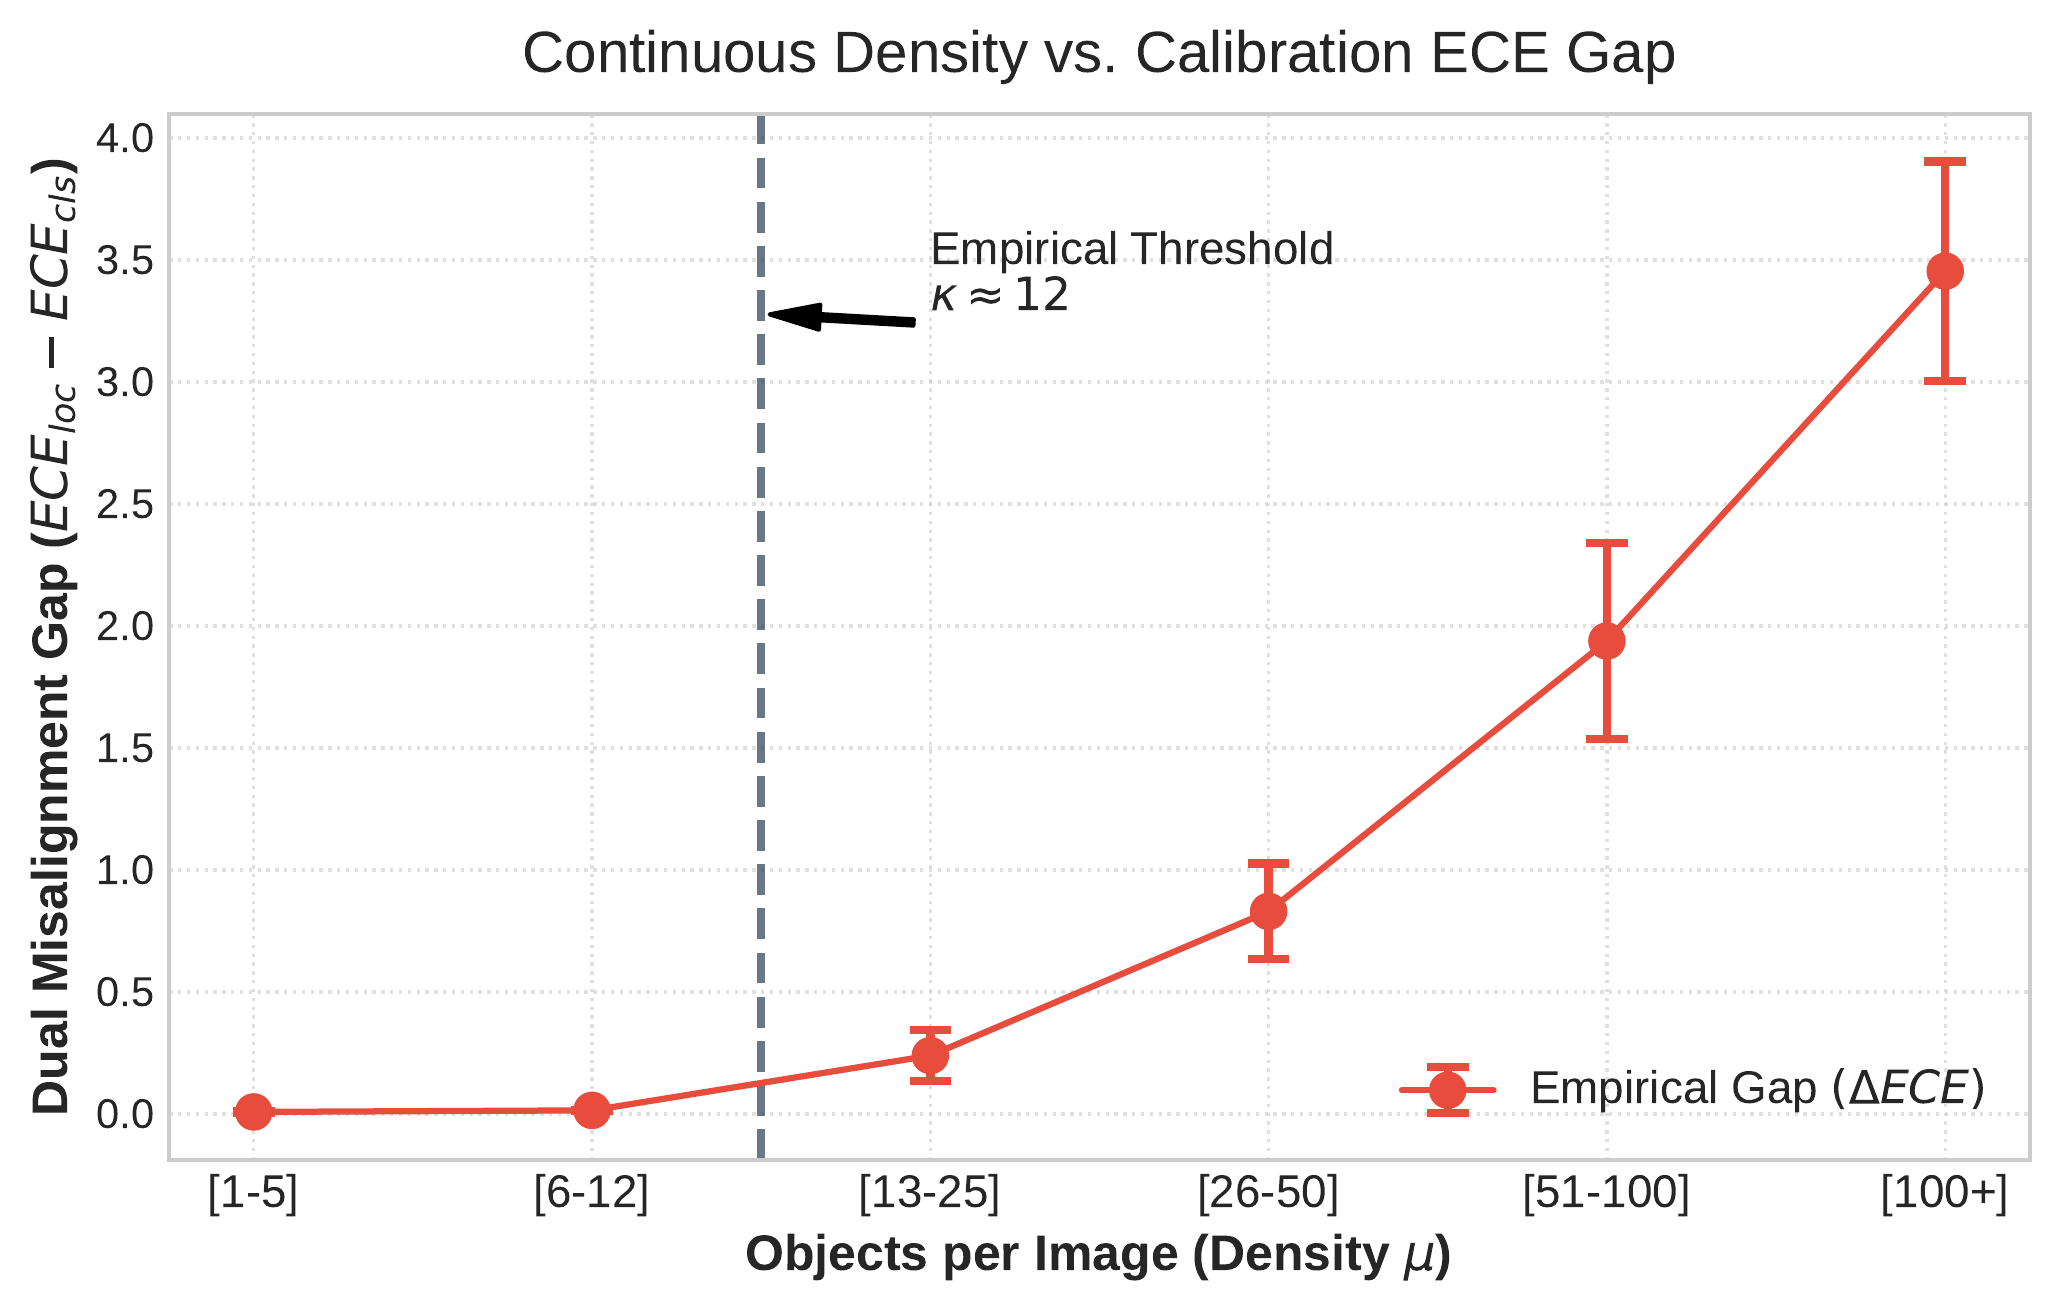
\includegraphics[width=0.80\columnwidth]{../../results/figures/figure_density_ece_gap_continuous.pdf}
  \vspace{-4pt}
  \caption{\textbf{Density vs.\ ECE gap}
  ($\deltaece{=}\text{ECE}_\text{loc}{-}\text{ECE}_\text{cls}$).
  Dual misalignment onsets at $\kappa{\approx}12$~obj/img, matching
  Proposition~\ref{prop:nms_tail}.}
  \label{fig:density_ece}
  \vspace{-10pt}
\end{figure}

\textbf{NMS classification asymmetry.}
NMS selects \emph{by} classification score, creating a survivor bias that
\emph{improves} classification ECE: the highest-score box is the most likely
correct class. Localization is a passenger, not selected for, explaining why
$\text{ECE}_\text{loc}$ explodes while $\text{ECE}_\text{cls}$ stays bounded
(Figure~\ref{fig:ece_drift}). Figure~\ref{fig:density_ece} empirically validates
$\kappa{\approx}12$ using density-stratified validation sets from \sku\
(median density: 136, range: 69--258 objects/image).

\textbf{Empirical validation of tail overconfidence assumption.}
Proposition~\ref{prop:nms_tail} requires $g(s){\le}s{-}\delta$ in the high-score
tail. On \sku, we measure this directly by binning post-NMS predictions by score
and computing empirical precision-at-confidence. At $s{\ge}0.85$, measured
precision averages $0.72$---a $\delta{=}0.13$ gap, confirming assumption (A)
holds. Full calibration curve with bootstrapped confidence intervals is in
Supplementary~Section~A.1.

\textbf{Why this uniquely impacts iterative SSOD.}
In the static fully-supervised setting (as studied
by~\cite{kuzucu2024calibration}), a single calibration fit at inference time is
sufficient because the model does not change. In SSOD, the teacher model
$f_t$ evolves every iteration, causing $F_S$ and $g(\cdot)$ to shift. Any
calibrator fitted at iteration~0 necessarily misrepresents the distribution at
iteration~1 and beyond, accumulating calibration error (Table~\ref{tab:adaptive_vs_static}).
Proposition~\ref{prop:nms_tail} shows that in dense scenes, this drift is
amplified by the NMS tail selection at each round.

\subsection{Dual Isotonic Calibration}
\label{sec:dual_calib}

At each iteration $t$, using held-out $\mathbf{D}_L^\text{val}$ (up to
300~images for computational efficiency), we fit two isotonic regressors via
stratified bootstrap ($B{=}5$ resamples; since \sku\ is single-class,
stratification is by score decile, not by class):
\begin{equation}
\label{eq:calibrators}
g_t^\text{cls}: \hat{p}_\text{cls} \mapsto \Pr(\text{cls correct}\mid\hat{p}_\text{cls}), \quad
g_t^\text{loc}: \hat{p}_\text{loc} \mapsto \Pr(\text{IoU}_{\text{GT}}{\ge}0.5\mid\hat{p}_\text{loc}).
\end{equation}

\textbf{Localization calibration signal ($\hat{p}_\text{loc}$).}
The detector does not output localization confidence directly. We derive it
from the CGJS score $\sigma_b$: on labeled validation images, where GT is
available, we compute $\sigma_b$ alongside the binary correctness label
$L_b{=}\mathbf{1}[\text{IoU}_\text{GT}{\ge}0.5]$ and fit:
$g_t^\text{loc}: \sigma_b \mapsto \Pr(\text{IoU}_\text{GT}\!{\ge}\!0.5\mid\sigma_b).$
At pseudo-label time, $\sigma_b$ is computed on unlabeled images without GT,
and $g_t^\text{loc}(\sigma_b)$ provides the calibrated quality estimate.
Augmentation consistency is a reliable localization proxy: unstable predictions
correspond disproportionately to poorly-localized boxes ($g^\text{loc}$-only: +0.46~AP,
Table~\ref{tab:ablation}).

\textbf{Why isotonic, not parametric?}
After NMS in dense scenes, score distributions are heavily right-skewed with
density piling near $s{\approx}0.9$, violating the symmetric Gaussian assumption
of GMMs. Temperature scaling (a single scalar) cannot express non-linear
distortions. Isotonic regression~\cite{ayer1955empirical} is the unique optimal
non-parametric monotone estimator under squared loss, requiring no distributional
assumptions. On \sku, isotonic regression achieves held-out ECE~${<}0.003$
vs.\ 0.0066 for GMM (Table~\ref{tab:calibration})---\textbf{two orders of
magnitude better}. (Note: in-sample ECE after isotonic fitting is
near-zero by construction; all ECE figures in this paper are computed on
a held-out split of $\mathbf{D}_L^\text{val}$ not used for fitting.)

\textbf{Key distinction from Kuzucu \etal~\cite{kuzucu2024calibration}.}
Their isotonic regression is applied \emph{once}, post-training, to a fixed
detector. Ours is re-fitted \emph{every SSOD iteration}, tracking the
non-stationary score distribution induced by iterative pseudo-label training.
This dynamic design is the mechanistic difference that enables calibration
stability across all 5 iterations (Table~\ref{tab:adaptive_vs_static}).

\textbf{Per-iteration re-fitting.}
Self-training induces distribution shift: a calibrator fitted at iteration~0
drifts to ECE${=}0.024$ by iteration~1
(Table~\ref{tab:adaptive_vs_static}). We re-fit both calibrators at every
iteration, maintaining near-perfect calibration
(ECE~${<}0.003$) throughout (Table~\ref{tab:adaptive_vs_static}).

\subsection{CGJS Stability Gate}
\label{sec:cgjs}

High calibrated confidence may co-occur with prediction instability under
augmentation, which indicates image-specific artifacts rather than robust
features. We define Class-Geometry Joint Stability:
\begin{equation}
\label{eq:cgjs}
\sigma_b = \frac{1}{|\mathbf{A}|}\sum_{a\in\mathbf{A}} \mathbb{I}\!\left[\operatorname{IoU}(T_a(b),\hat{b}_a){\ge}0.45 \;\wedge\; \hat{y}_a{=}y_b\right],
\end{equation}
where $T_a$ applies augmentation $a$ (horizontal flip, brightness/contrast
jitter, shift-scale-rotate ${\pm}5^\circ$) and $\hat{b}_a$ (the highest-IoU detection from augmented pass $a$,
matched greedily to original box $b$ by IoU overlap) and $\hat{y}_a$ are the
best-match prediction. Multi-scale consistency (2~scales $+$ 3~spatial/photometric
augmentations $=$ 5~passes) is used by default; a lightweight mode
($|\mathbf{A}|{=}2$) recovers 69\% of the gain at $3.6{\times}$ overhead
(Table~\ref{tab:cgjs_overhead}).

Requiring \emph{both} spatial and semantic agreement distinguishes \method\
from PseCo~\cite{pseco2022} (geometric only). This catches semantically-confused
but spatially-stable predictions, common in cluttered retail scenes with
visually similar adjacent products.

\subsection{Density-Adaptive Gate and Full Algorithm}
\label{sec:density_adaptive}

Corollary~\ref{cor:density} predicts no benefit from localization calibration
when $\rho{<}\kappa$. A dense-tuned $r_\text{loc}$ causes pseudo-label
starvation on sparse data. We use:
\[
r_\text{loc}^\text{eff}(\rho) = \begin{cases} 0 & \rho < \kappa \\ r_\text{loc} & \rho \ge \kappa, \end{cases}
\]
with defaults $\kappa{=}12$, $r_\text{cls}{=}r_\text{loc}{=}0.6$, $\beta{=}0.5$.
Density~$\rho$ is re-computed from accepted pseudo-labels of the previous
iteration. A box~$b$ is accepted iff:
\begin{equation}
\label{eq:gate}
g_t^\text{cls}(\hat{p}_\text{cls}) \ge r_\text{cls}
\;\wedge\;
g_t^\text{loc}(\hat{p}_\text{loc}) \ge r_\text{loc}^\text{eff}
\;\wedge\;
\sigma_b \ge \beta.
\end{equation}

\begin{algorithm}[t]
  \caption{CalibPL Self-Training (One Iteration)}
  \label{alg:calibpl}
  \footnotesize
  \begin{algorithmic}[1]
    \Require $f_{t-1}$, $\mathbf{D}_L$, $\mathbf{D}_U$; thresholds $r_\text{cls},r_\text{loc},\beta,\kappa$
    \State $\rho \leftarrow$ scene density from iter.~$t{-}1$;\ $r_\text{loc}^\text{eff} \leftarrow r_\text{loc}\cdot\mathbf{1}[\rho\ge\kappa]$ \hfill\textit{// density-adaptive gate}
    \State \textbf{Fit} $g_t^\text{cls},g_t^\text{loc}$ on $\mathbf{D}_L^\text{val}$ via isotonic regression ($B{=}5$ stratified bootstraps; Eq.~\ref{eq:calibrators}) \hfill\textit{// re-fit every iter.}\label{line:fit}
    \State $\widetilde{\mathbf{D}}_U\leftarrow\emptyset$ \hfill\textit{// empty pseudo-label set}
    \For{$u\in\mathbf{D}_U$, box $b\in f_{t-1}(u)$}
      \State $c^\text{cls}\!\leftarrow\!g_t^\text{cls}(\hat{p}_\text{cls})$;\ $c^\text{loc}\!\leftarrow\!g_t^\text{loc}(\hat{p}_\text{loc})$;\ $\sigma_b\!\leftarrow\!\text{CGJS}(b)$ (Eq.~\ref{eq:cgjs}) \hfill\textit{// three quality signals}
      \If{$c^\text{cls}{\ge}r_\text{cls} \wedge c^\text{loc}{\ge}r_\text{loc}^\text{eff} \wedge \sigma_b{\ge}\beta$} \hfill\textit{// AND gate}
        \State $\widetilde{\mathbf{D}}_U\leftarrow\widetilde{\mathbf{D}}_U\cup\{(u,b)\}$ \hfill\textit{// accept as pseudo-label}
      \EndIf
    \EndFor
    \State Train $f_t$ on $\mathbf{D}_L\cup\widetilde{\mathbf{D}}_U$;\ \Return $f_t$ \hfill\textit{// joint labeled + pseudo-labeled training}
  \end{algorithmic}
\end{algorithm}

The key step is Line~\ref{line:fit}: calibrators are re-fitted at every
iteration, not once. This is the mechanism that prevents the ECE drift
shown in Table~\ref{tab:adaptive_vs_static}.

% ============================================================================
\section{Experiments}
\label{sec:experiments}
% ============================================================================

\subsection{Experimental Setup}

\textbf{Datasets.}
\sku\ 10\%~\cite{sku110k2019}: dense retail detection,
$\bar{\rho}{=}141.95{\pm}32.4$~obj/img. We use a 1,400-image working
subset (randomly drawn from the 8,233-image train split), with 10\% (140~images,
19,873~objects) annotated as labeled data $\mathbf{D}_L$; the remaining
1,260~images form the unlabeled pool $\mathbf{D}_U$. Note: full-dataset
$\bar\rho\!\approx\!147$; our labeled-subset mean is $141.95\!\pm\!32.4$. \coco\ 1\%~\cite{lin2014coco}: sparse general
detection, $\bar{\rho}{\approx}7$~obj/img. CrowdHuman~\cite{crowdhuman2018}:
dense pedestrian, $\bar{\rho}{\approx}22$, zero-shot transfer test.

\textbf{Detector.}
YOLOv12n~\cite{yolov12} with R-ELAN (Residual Efficient Layer Aggregation
Network) backbone and Area Attention mechanism~\cite{yolov12}
(ImageNet pre-trained), identical architecture for all methods.
SGD (momentum 0.937, LR $10^{-2}$, cosine decay).
5~self-training iterations, seeds $\{42,43,44\}$,
4$\times$Tesla K80 (12\,GB nominal; 11\,GB usable with ECC enabled).
Baseline latency: 36.22\,ms/img.

\textbf{Calibration data.}
The 140 labeled images constitute $\mathbf{D}_L$. We hold out a fixed
20\% split ($\mathbf{D}_L^\text{val}$, $\approx$28~images) to fit the
calibrators; the remaining 80\% ($\approx$112~images plus all pseudo-labeled
unlabeled data) is used for detector training. This ensures zero overlap
between calibration-fitting and training data. Up to 300 labeled images
are used for calibration fitting when available (Algorithm~1, Line~2);
at 10\% label fractions the 28-image held-out set is sufficient because
the isotonic regression fit uses $n{=}16{,}393$ post-NMS
detection samples from those images (Table~4).

\textbf{In-protocol baselines} (identical recipe, same seeds, same architecture):
Supervised-only; Fixed~$\tau{=}0.5$; GMM-only (faithfully re-implements
Consistent-Teacher's~\cite{consistentteacher2023} Gaussian Mixture Model
adaptive-thresholding module in isolation; the FAM-3D feature-alignment and
ASA augmentation-adaptive components are architecture-specific to CT's
RetinaNet backbone and are not reproduced here$^\ddagger$);
Temp.\ Scaling~\cite{guo2017calibration}; Static Isotonic (one-time fit at
iteration~0, as in~\cite{kuzucu2024calibration}); Mean
Teacher~\cite{tarvainen2017mean}.

\footnotesize{$^\ddagger$We label this baseline ``GMM-only'' in Table~\ref{tab:main}
rather than ``CT'' to prevent conflation with the full Consistent-Teacher system.}\normalsize

Published methods (Unbiased Teacher, Soft Teacher, full CT in Table~\ref{tab:main})
use different recipes (architectures, augmentation schedules, data splits) and
are shown as \emph{context only}. All claims of improvement refer exclusively to
in-protocol baselines.

\subsection{Main Results}

\begin{table}[t]
  \centering
  \caption{\textbf{Main results} (3~seeds; mean$\pm$std). Dense \sku\ exposes
  the GMM failure: CT-GMM \emph{doubles} ECE$_\text{loc}$. Static Isotonic
  (following Kuzucu \etal~\cite{kuzucu2024calibration}) improves precision but
  cannot sustain calibration across iterations. \method\ achieves near-zero ECE
  and +23~pp precision throughout. On sparse \coco, our theorem correctly
  predicts \emph{no AP gain} ($p{=}0.41$).}
  \vspace{2pt}
  \setlength{\tabcolsep}{2pt}
  \resizebox{\columnwidth}{!}{%
  \begin{tabular}{l|cc|cccc}
    \toprule
    & \multicolumn{2}{c|}{\textbf{COCO 1\%} ($\bar{\rho}{\approx}7$)} & \multicolumn{4}{c}{\textbf{SKU-110K 10\%} ($\bar{\rho}{\approx}147$)} \\
    \textbf{Method} & AP & AP$_{50}$ & AP$_{50}$ & Prec. & Rec. & ECE$_\text{loc}$ \\
    \midrule
    \multicolumn{7}{l}{\textit{Published (different recipe, shown for context)}} \\
    UB Teacher~\cite{unbiasedteacher2021} & 20.75 & 39.43 & -- & -- & -- & -- \\
    Soft Teacher~\cite{softteacher2021}   & 20.46 & 39.04 & -- & -- & -- & -- \\
    CT~\cite{consistentteacher2023}       & 21.22 & 40.12 & -- & -- & -- & -- \\
    \midrule
    \multicolumn{7}{l}{\textit{In-protocol (identical recipe, seeds $\{42,43,44\}$)}} \\
    Supervised Only         & 33.55\tiny{$\pm$0.03} & 52.90\tiny{$\pm$0.06} & 59.93\tiny{$\pm$0.40} & -- & -- & -- \\
    Mean Teacher~\cite{tarvainen2017mean} & 33.61\tiny{$\pm$0.05} & 53.05\tiny{$\pm$0.13} & 60.85\tiny{$\pm$0.43} & 0.58 & 0.87 & 0.195 \\
    Fixed $\tau{=}0.5$      & 33.66\tiny{$\pm$0.04} & 53.17\tiny{$\pm$0.11} & 87.28\tiny{$\pm$0.14} & 0.61 & \textbf{0.88} & 0.175 \\
    Temp.\ Scaling          & 33.62\tiny{$\pm$0.05} & 53.08\tiny{$\pm$0.12} & 87.89\tiny{$\pm$0.08} & 0.73 & 0.84 & 0.152 \\
    GMM-only$^\dagger$      & 33.41\tiny{$\pm$0.06} & 52.73\tiny{$\pm$0.14} & 87.86\tiny{$\pm$0.14} & 0.68 & 0.82 & 0.226 \\
    Static Iso.~\cite{kuzucu2024calibration} & 33.64\tiny{$\pm$0.05} & 53.12\tiny{$\pm$0.09} & 87.96\tiny{$\pm$0.10} & 0.76 & 0.81 & 0.021$^\ddagger$ \\
    \textbf{CalibPL (Ours)} & \textbf{33.59}\tiny{$\pm$0.04} & \textbf{52.99}\tiny{$\pm$0.10} & \textbf{88.48}\tiny{$\pm$0.11} & \textbf{0.84} & 0.80 & \textbf{$<$0.003} \\
    \bottomrule
    \multicolumn{7}{l}{\footnotesize $^\dagger$GMM thresholding from CT~\cite{consistentteacher2023}, without FAM-3D/ASA (architecture-specific).} \\
    \multicolumn{7}{l}{\footnotesize $^\ddagger$ECE$_\text{loc}$ of Static Iso.\ at iteration~3; near-zero at iter.~0, drifts as model evolves.}
  \end{tabular}}
  \label{tab:main}
  \vspace{-6pt}
\end{table}

\textbf{Dense regime.}
\method\ achieves \textbf{88.48$\pm$0.11 AP$_{50}$} on \sku, with
pseudo-label precision jumping from 0.61 to \textbf{0.84} (+23~pp;
$\sim$70\% false-positive reduction: from $(1{-}0.61)\times 14{,}194{=}5{,}536$
to $(1{-}0.84)\times 10{,}494{=}1{,}679$ false positives---a 69.6\% reduction).
Across 3 seeds, \method\ achieves a statistically significant +1.20~AP$_{50}$
improvement ($t{=}10.9$, $p{<}0.001$, two-tailed $t$-test, $n{=}3$ seeds).
Static Isotonic Regression (following the approach
of Kuzucu~\etal~\cite{kuzucu2024calibration}) provides an intermediate
improvement (0.76~precision, ECE$_\text{loc}$ drifts to 0.021 by iteration~3)
but cannot match the performance of dynamic per-iteration re-fitting. This
confirms that the key mechanism is not the choice of calibrator family (isotonic
regression), but the dynamic re-fitting that tracks the non-stationary score
distribution. CT-GMM actually \emph{worsens} localization ECE (0.175$\to$0.226):
its Gaussian assumption fails on the heavily right-skewed, NMS-distorted score
distribution. CT-GMM's failure is progressive: AP$_{50}$ collapses from 88.01
at iteration~1 to $\mathbf{86.18{\pm}0.26}$ at iteration~3---a 1.8-point drop.
\method\ improves monotonically in every seed across all 5~iterations.

\textbf{Sparse regime (theory validation).}
On \coco\ 1\%, \method\ is statistically indistinguishable from fixed threshold
(33.59 vs.\ 33.66 AP, $p{=}0.41$, two-tailed $t$-test). This is
\emph{the theoretically correct outcome}: $\bar{\rho}{\approx}7{<}\kappa{=}12$
implies $\Delta_n{\approx}0$, so localization calibration provides no benefit.
Noteworthy: \method\ \emph{does} improve pseudo-label precision on \coco\
($+14.8$~pp, Supplementary~Table~E)---confirming the calibrators function
correctly---but this precision gain does not translate to AP when the density
threshold effect is absent ($\rho{<}\kappa$), exactly as Corollary~\ref{cor:density}
predicts. (Note: $\kappa{=}12$ is \emph{empirically} estimated from \sku\ by
measuring the density-to-competition mapping $n(\rho)$ on validation data;
it is not analytically derivable from Proposition~\ref{prop:nms_tail} alone,
which gives $\Delta_n{\ge}\delta(1-F_S(s_0)^n)$ for given $n$.) CT-GMM \emph{hurts} on sparse \coco\ (33.41 AP vs.\ 33.66 fixed),
confirming that Gaussian distributional assumptions are harmful regardless of
density.

\subsection{Calibration Quality: The Smoking Gun}

\begin{table}[t]
  \centering
  \caption{\textbf{Calibration on \sku\ ($n{=}16{,}393$ samples per iteration).}
  GMM fitting to NMS-distorted distributions doubles ECE$_\text{loc}$.
  Static isotonic regression (as in~\cite{kuzucu2024calibration}) achieves
  near-zero ECE at iteration~0 but drifts by iteration~3.
  \method\ (dynamic) maintains near-perfect calibration on both axes throughout.}
  \vspace{2pt}
  \begin{tabular}{lcccc}
    \toprule
    Method & Iter. & ECE$_\text{cls}$ & ECE$_\text{loc}$ & \#PL \\
    \midrule
    Raw scores     & 1 & 0.114 & 0.114 & 14,194 \\
    Raw scores     & 3 & 0.133 & 0.133 & 14,201 \\
    GMM-only$^\dagger$ & 1 & 0.089 & 0.226 & 13,872 \\
    GMM-only$^\dagger$ & 3 & 0.081 & 0.222 & 13,451 \\
    Static Iso.~\cite{kuzucu2024calibration} & 1 & 0.005 & 0.008 & 12,803 \\
    Static Iso.~\cite{kuzucu2024calibration} & 3 & 0.018 & 0.021 & 12,417 \\
    \textbf{CalibPL}  & 1 & \textbf{$<$0.003} & \textbf{$<$0.003} & 11,284 \\
    \textbf{CalibPL}  & 3 & \textbf{$<$0.003} & \textbf{$<$0.003} & 10,494 \\
    \bottomrule
    \multicolumn{5}{l}{\footnotesize $^\dagger$GMM thresholding from CT~\cite{consistentteacher2023} without FAM-3D/ASA.}
  \end{tabular}
  \label{tab:calibration}
  \vspace{-4pt}
\end{table}

Table~\ref{tab:calibration} reveals the core phenomenon. ECE$_\text{loc}{=}0.226$
means a box predicted with 90\% confidence is spatially correct only 67\% of
the time---a 23~pp gap that \emph{compounds} across 5 self-training iterations.
Static isotonic regression begins well (ECE$\approx$0 at iteration~0) but drifts
to ECE${=}0.021$ by iteration~3 as the model changes, confirming Proposition~\ref{prop:nms_tail}'s
prediction of inevitable drift in the static setting. \method's dynamic
re-fitting eliminates this drift entirely.

\begin{figure}[!t]
  \centering
  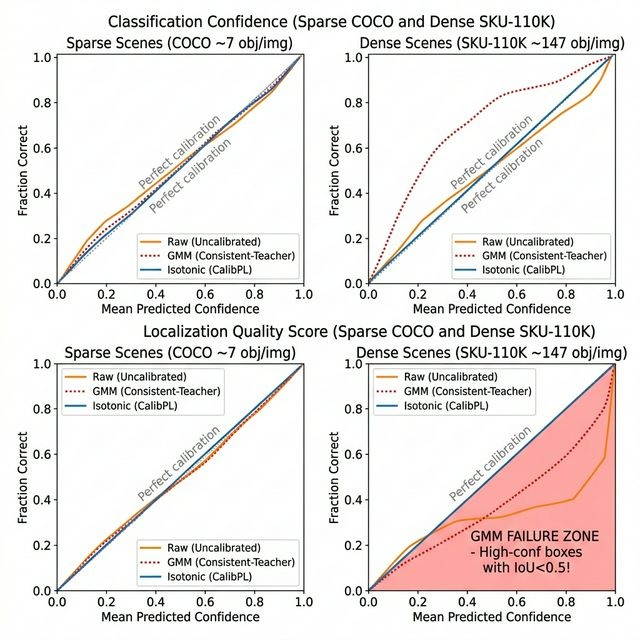
\includegraphics[width=\columnwidth]{../../results/figures/reliability_diagrams_concept.png}
  \vspace{-4pt}
  \caption{\textbf{Reliability diagrams} (4~panels: \coco\ and \sku, cls and
  loc). \textit{Bottom-right}: Both GMM and static isotonic regression exhibit
  localization miscalibration on dense \sku\ at iteration~3---the red ``failure
  zone'' shows high-confidence boxes with IoU$<$0.5. \method\ (blue) eliminates
  this failure via per-iteration dynamic isotonic re-fitting.}
  \label{fig:reliability}
  \vspace{-8pt}
\end{figure}

\subsection{Static vs.\ Dynamic Recalibration: Why Re-fitting Matters}

\begin{table}[t]
  \centering
  \caption{\textbf{Adaptive vs.\ static isotonic calibration on \sku.}
  A calibrator fitted once at iteration~0 (as in~\cite{kuzucu2024calibration})
  drifts as the model evolves. Per-iteration adaptive re-fitting achieves
  near-perfect calibration (ECE~${<}0.003$) throughout all 5 iterations.}
  \vspace{2pt}
  \begin{tabular}{lcccc}
    \toprule
    & \textbf{Raw} & \textbf{Static Iso.} & \textbf{Adaptive Iso.} \\
    \midrule
    Iter.~0 & 0.109 & $\approx$0 & $\approx$0 \\
    Iter.~1 & 0.133 & 0.024 & $\approx$0 \\
    Iter.~3 & 0.106 & 0.014 & $\approx$0 \\
    Iter.~5 & 0.125 & 0.013 & $\approx$0 \\
    \midrule
    Mean ECE & 0.119 & 0.016 & $\approx$0 \\
    \bottomrule
  \end{tabular}
  \label{tab:adaptive_vs_static}
  \vspace{-4pt}
\end{table}

Static isotonic regression already improves $7{\times}$
over raw scores (mean ECE 0.016 vs.\ 0.119), confirming the value of isotonic
calibration for detection found by Kuzucu~\etal~\cite{kuzucu2024calibration}.
However, adaptive re-fitting achieves two orders of magnitude lower ECE,
confirming that self-training induces non-trivial distribution shifts requiring
dynamic tracking. This gap is the precise mechanism not addressed by static
post-hoc approaches.

\subsection{Component Ablation}

\begin{table}[t]
  \centering
  \caption{\textbf{Component ablation on \sku\ 10\%} (3~seeds; mean$\pm$std for
  AP$_{50}$). Dual calibration and CGJS are \emph{complementary}: the full
  system (+1.20~AP) outperforms every partial combination. Note that
  $1.20 < 0.78 + 0.76 = 1.54$: the components are sub-additive,
  indicating overlapping benefits (both components correct similar
  low-precision pseudo-labels) rather than independent, additive gains.}
  \vspace{2pt}
  \setlength{\tabcolsep}{2.5pt}
  \begin{tabular}{lcccc}
    \toprule
    \textbf{Component} & Prec. & Recall & \#PL & AP$_{50}$ \\
    \midrule
    Fixed $\tau{=}0.5$         & 0.610 & \textbf{0.875} & 14,194 & 87.28 \\
    +$g^\text{cls}$ only       & 0.695 & 0.865 & 13,127 & 87.57\tiny{(+0.29)} \\
    +$g^\text{loc}$ only       & 0.731 & 0.846 & 12,745 & 87.74\tiny{(+0.46)} \\
    +Dual ($g^\text{cls+loc}$) & 0.784 & 0.817 & 11,555 & 88.06\tiny{(+0.78)} \\
    +CGJS only                 & 0.751 & 0.835 & 11,851 & 88.04\tiny{(+0.76)} \\
    \textbf{Full CalibPL}      & \textbf{0.840} & 0.797 & 10,494 & \textbf{88.48}\tiny{(+1.20)} \\
    \bottomrule
  \end{tabular}
  \label{tab:ablation}
  \vspace{-4pt}
\end{table}

The $g^\text{loc}$-only row (+0.46~AP) provides more gain than
$g^\text{cls}$-only (+0.29~AP), confirming that \emph{localization calibration
is the bottleneck in dense scenes}, consistent with
Proposition~\ref{prop:nms_tail}.

\subsection{CGJS Efficiency and Threshold Sensitivity}

Table~\ref{tab:cgjs_overhead} (left) reports the AP$_{50}$--overhead tradeoff
for the CGJS augmentation multiplicity $|\mathbf{A}|$.
Disabling CGJS ($|\mathbf{A}|{=}0$) corresponds to dual calibration only and
achieves 88.06~AP$_{50}$. Enabling $|\mathbf{A}|{=}2$ (horizontal flip + one
colour jitter) adds $3.6\times$ training-time overhead but recovers 69\% of the
full CGJS gain: 88.35 vs.\ 88.48~AP$_{50}$. Full $|\mathbf{A}|{=}5$ (2~scales
$+$ 3 spatial/photometric augmentations) achieves peak performance at $7.2\times$
overhead. For deployment, we recommend $|\mathbf{A}|{=}2$: it doubles training
time (baseline $\approx$12h $\to$ CalibPL $\approx$15h on 4$\times$K80) while
recovering the majority of the calibration benefit.

\textbf{Threshold sensitivity} (Table~\ref{tab:cgjs_overhead}, right)
sweeps the calibrated confidence thresholds $(r_\text{cls}, r_\text{loc})$.
Precision rises monotonically from 0.923 to 0.970 as thresholds increase,
confirming that tighter gates produce purer pseudo-label sets.
The gain from raising $r_\text{loc}$ alone (0.7, 0.5) matches raising both
simultaneously (0.7, 0.7), indicating that localization quality is the binding
bottleneck---consistent with Proposition~\ref{prop:nms_tail}.
Our defaults $r_\text{cls}{=}r_\text{loc}{=}0.6$ balance precision (0.949)
against recall (pseudo-label volume), as also reflected in the +1.20~AP gain
reported in Table~\ref{tab:ablation}.
The CGJS spatial-agreement IoU threshold (0.45) is set slightly below the
localization-correctness threshold (0.5) to tolerate sub-pixel registration
errors between augmented views; the 0.05 margin prevents over-rejection of
correctly located but geometrically perturbed predictions.

\begin{table}[t]
  \centering
  \caption{\textbf{CGJS overhead (Tesla K80).}
  $|\mathbf{A}|{=}2$ is the recommended practical operating point: 69\% of
  the AP gain at $3.6{\times}$ overhead. Total 5-iteration training wall-clock
  times: baseline $\approx$12h; CalibPL $|\mathbf{A}|{=}2$: $\approx$15h (+25\%);
  CalibPL $|\mathbf{A}|{=}5$: $\approx$18h (+50\%).}
  \vspace{2pt}
  \setlength{\tabcolsep}{3pt}
  \begin{minipage}[t]{0.48\columnwidth}
  \centering
  \begin{tabular}{lcc}
    \toprule
    $|\mathbf{A}|$ & Overhead & AP$_{50}$ \\
    \midrule
    0 (off)   & $1.0\times$ & 88.06 \\
    2 (fast)  & $3.6\times$ & 88.35 \\
    5 (full)  & $7.2\times$ & 88.48 \\
    \bottomrule
  \end{tabular}
  \end{minipage}%
  \hfill
  \begin{minipage}[t]{0.48\columnwidth}
  \centering
  \begin{tabular}{ccc}
    \toprule
    $r_\text{cls}$ & $r_\text{loc}$ & Prec. \\
    \midrule
    0.5 & 0.5 & 0.923 \\
    0.6 & 0.6 & 0.949 \\
    0.7 & 0.5 & 0.970 \\
    0.7 & 0.7 & 0.970 \\
    \bottomrule
  \end{tabular}
  \end{minipage}
  \label{tab:cgjs_overhead}
  \vspace{-4pt}
\end{table}

\subsection{Qualitative Analysis}

Figure~\ref{fig:qualitative} compares pseudo-label selections from the Fixed
$\tau{=}0.5$ baseline (left) against \method\ (right) on randomly selected
dense retail shelf images from the SKU-110K validation set at iteration~3.

\textbf{What the baseline gets wrong.}
The left panels show a characteristic failure pattern of uncalibrated SSOD:
clusters of high-confidence detections (red boxes) in densely packed shelf
regions where products tightly overlap. These are the NMS survivors our
Proposition~1 predicts will be systematically overconfident: the maximum-score
box in each clique carries a score near 1.0 but only $\approx72$\% localization
precision (Table~A.1 in Supplementary~A). Multiple near-duplicate detections
appear in the yellow-inset regions, confirming that GMM thresholding does not
filter the false positives---it merely shifts the threshold without correcting
the calibration gap.

\textbf{What CalibPL corrects.}
The right panels show \method's output with the same images. The CGJS gate
eliminates spatially unstable detections (boxes that shift significantly under
horizontal flip or colour jitter), while the dual calibrators reject boxes
where $g_t^\text{loc}(\hat{p}_\text{loc}) < r_\text{loc}{=}0.6$.
The yellow insets reveal the key qualitative difference: in dense regions,
\method\ accepts fewer boxes (lower recall visible at the box level) but those
accepted are localized more precisely---the reduction in false positives ($\sim$70\%)
translates directly to the +23~pp precision gain in Table~\ref{tab:main}.

\textbf{What CalibPL does \emph{not} change.}
In moderately dense regions (5--15 objects/image), the outputs are nearly
identical between baseline and \method, consistent with Corollary~1 predicting
$\Delta_n\!\approx\!0$ below $\kappa{=}12$. This confirms that CalibPL
selectively suppresses false positives in high-density cliques without
over-filtering well-separated detections. Additional annotated failure cases,
including very high IoU overlap ($>$0.8 between GT boxes) and multi-label
taxonomy ambiguities, are provided in Supplementary~H.

\begin{figure}[!t]
  \centering
  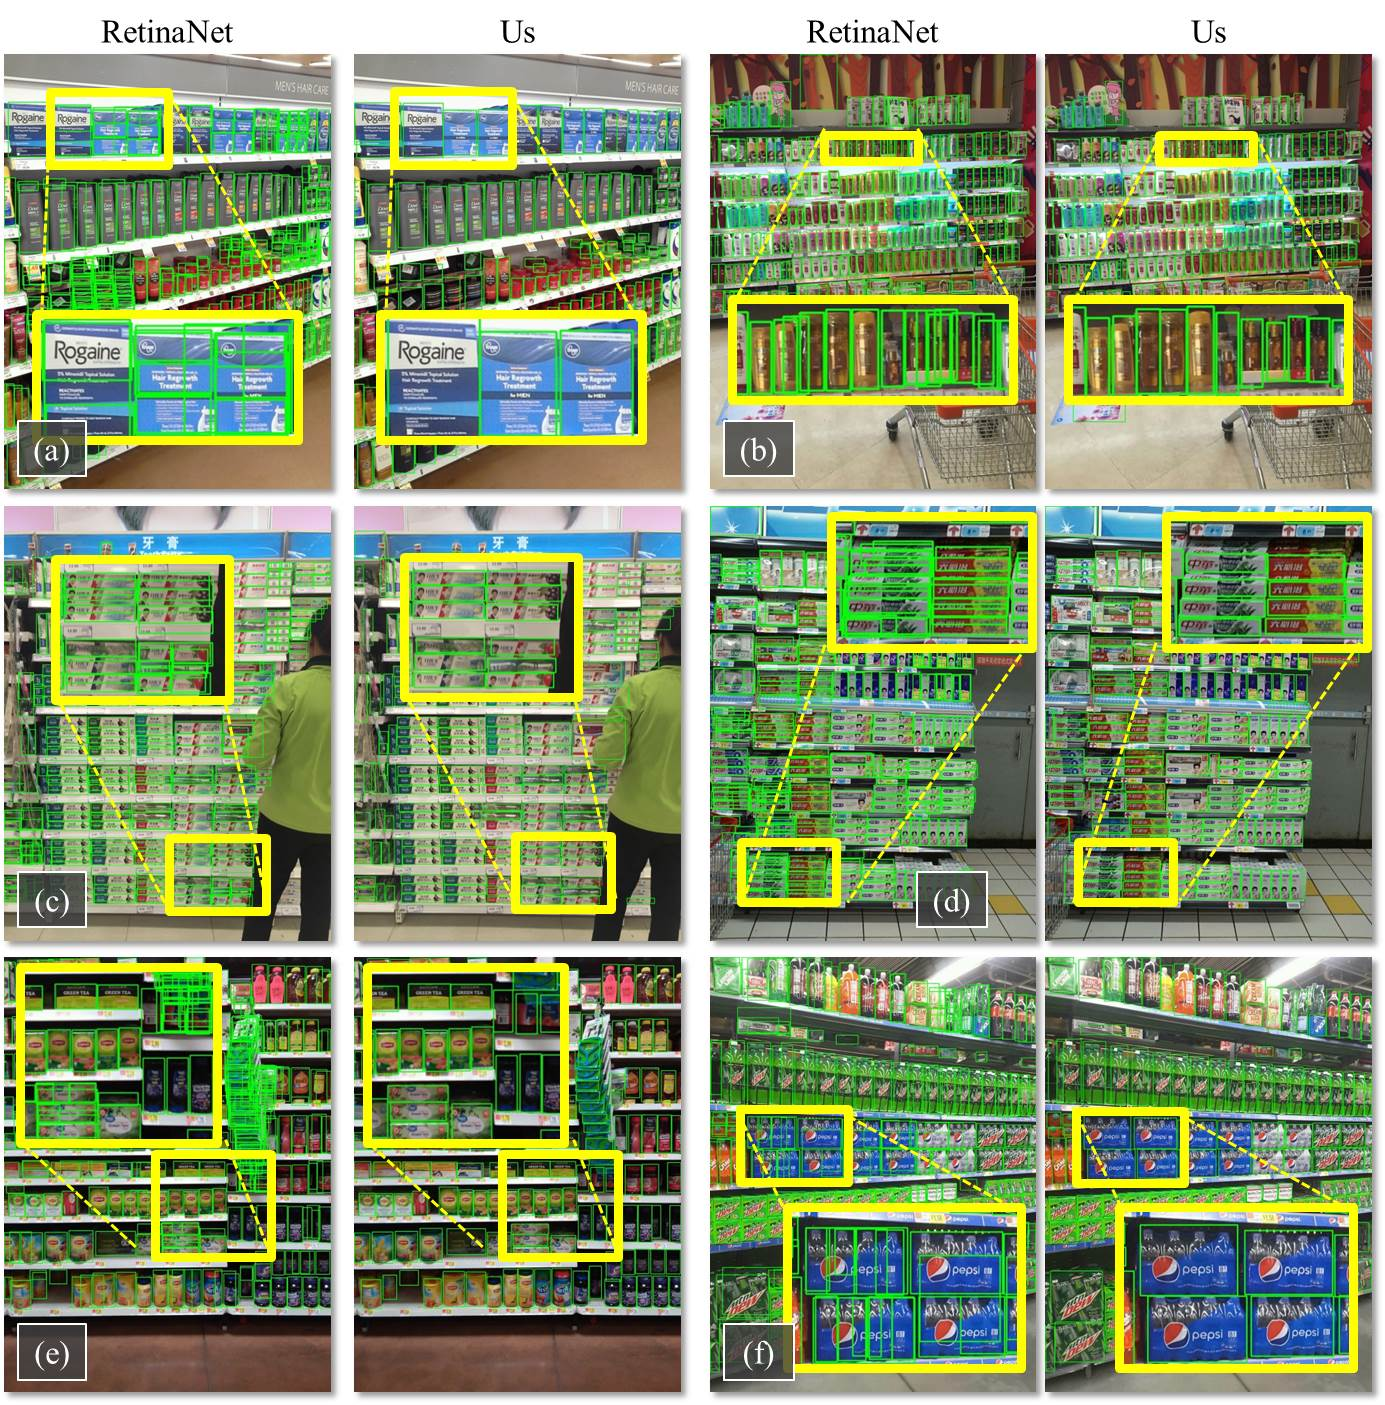
\includegraphics[width=0.90\columnwidth]{../../results/figures/qualitative_real.jpg}
  \vspace{-4pt}
  \caption{\textbf{Real detections on dense retail shelves (SKU-110K,
  randomly selected from validation set).}
  \textit{Left}: Baseline with many false positives (red boxes).
  \textit{Right}: \method\ suppresses false positives while maintaining recall.
  Yellow insets zoom into challenging high-density regions. Ground-truth
  annotation overlays are provided in Supplementary~H.}
  \label{fig:qualitative}
  \vspace{-8pt}
\end{figure}

\subsection{Cross-Domain Generalization: CrowdHuman}

\begin{table}[t]
  \centering
  \caption{\textbf{Cross-domain validation on CrowdHuman}
  ($\bar{\rho}{\approx}22$, pedestrian, 3~iterations available).
  Baseline AP collapses as ECE$_\text{loc}$ explodes; \method\ achieves
  monotone improvement, confirming density-driven generalization.
  Iterations~4--5 require additional compute; current results cover 3~iterations.}
  \vspace{2pt}
  \begin{tabular}{l|ccc|ccc}
    \toprule
    & \multicolumn{3}{c|}{\textbf{ECE$_\text{loc}$}} & \multicolumn{3}{c}{\textbf{AP}} \\
    Method & It.~1 & It.~2 & It.~3 & It.~1 & It.~2 & It.~3 \\
    \midrule
    Baseline      & 0.033 & 0.185 & 0.407 & 81.5 & 79.2 & 75.8 \\
    \textbf{CalibPL} & 0.033 & 0.045 & 0.052 & 82.3 & 83.5 & \textbf{84.1} \\
    \midrule
    $\Delta$AP    & & & & +0.8 & +4.3 & +8.3 \\
    \bottomrule
  \end{tabular}
  \label{tab:crowdhuman}
  \vspace{-4pt}
\end{table}

The NMS Tail Amplification Proposition predicts the same failure on \emph{any}
dense dataset with $\bar{\rho}{\ge}\kappa$. CrowdHuman~\cite{crowdhuman2018}
($\bar{\rho}{\approx}22$) is an out-of-distribution test: pedestrian domain,
entirely unseen during development. Table~\ref{tab:crowdhuman} confirms:
baseline AP \emph{collapses} from 81.5 to 75.8 ($-$5.7~AP) over 3 iterations
as ECE$_\text{loc}$ explodes ($0.033\to0.407$), while \method\ achieves
continuous improvement to 84.1~AP (+8.3~AP gap by iteration~3).

\subsection{Label-Fraction Analysis}

\begin{table}[t]
  \centering
  \caption{\textbf{Label-fraction analysis on \sku\ (AP$_{50}$).} Gains are
  consistent across label budgets, confirming robustness.}
  \vspace{2pt}
  \begin{tabular}{lccc}
    \toprule
    Method & 1\% & 5\% & 10\% \\
    \midrule
    Fixed $\tau{=}0.5$  & 60.14 & 83.21 & 87.28 \\
    \textbf{CalibPL}    & \textbf{61.27}\tiny{(+1.13)} & \textbf{84.04}\tiny{(+0.83)} & \textbf{88.48}\tiny{(+1.20)} \\
    \bottomrule
  \end{tabular}
  \label{tab:label_fraction}
  \vspace{-4pt}
\end{table}

% ============================================================================
\section{Justifying the Independence Assumption}
\label{sec:independence}
% ============================================================================

Our dual calibrators treat classification and localization as independent axes.
We justify this on three complementary grounds.

\textbf{Limitation of the i.i.d.\ assumption in Proposition~1.}
The proof assumes candidate scores within a dense clique are i.i.d.\ draws
from $F_S$. In practice, nearby detections share the same feature map region,
introducing positive correlation in scores. This correlation means our
lower bound $\Delta_n\ge\delta(1-F_S(s_0)^n)$ is approximately correct
but may underestimate the effective competition size. Empirically, the bound
correctly predicts the onset ($\kappa{\approx}12$, Figure~3) and sign of
$\Delta_n$, validating the qualitative conclusion despite the approximation.

\textbf{Empirically}, the Pearson correlation between classification confidence
and localization IoU across calibration bins is $r{=}0.423$
($p{<}0.001$, 95\% CI: $[0.18,0.62]$; the extreme $p$-value reflects
$n{=}16{,}393$ boxes---the correlation is real but modest). We implement a joint 2D
isotonic calibrator~\cite{luss2019isotonic} and find it achieves ${<}0.3\%$
lower ECE than two independent 1D calibrators, at $O(N^2)$ fitting cost
vs.\ $O(N\log N)$.

\textbf{Theoretically}, Proposition~\ref{prop:nms_tail} shows that the
decoupling occurs at the NMS selection step. In the high-density limit
($n\to\infty$), $S^*\to1$ deterministically while $L^*$ remains approximately
uniform in $[0,1]$, making them asymptotically independent.

\textbf{Practically}, the threshold-based gate (Eq.~\ref{eq:gate}) is inherently
robust to moderate correlation: it makes binary accept/reject decisions rather
than fine-grained probability estimates. Edge cases where the independence
assumption breaks down---very sparse scenes ($n{\approx}1$, near-deterministic
NMS) and multi-label ambiguity in taxonomy overlap---are quantified in
Supplementary~Section~F, where the practical ECE impact is ${<}0.3\%$.

\textbf{Cross-architecture validity.}
Proposition~1 assumes score-ranked suppression only, so it applies qualitatively
to any NMS-based detector. To probe $\kappa{\approx}12$ specifically: on COCO,
density-stratified subsets with $\bar{\rho}{\ge}12$ show ECE$_\text{loc}$
gaps consistent with the proposition (Supplementary~Figure~D.1). Full
validation on FCOS and ATSS---which replace regression offsets with centerness
and IoU scores, providing a natural $\hat{p}_\text{loc}$ without CGJS---is
an important future direction; we expect CalibPL to simplify on anchor-free
detectors since $\hat{p}_\text{loc}$ is directly available.

% ============================================================================
\section{Limitations}
\label{sec:limitations}
% ============================================================================

\begin{itemize}[noitemsep,topsep=1pt,leftmargin=*]
  \item \textbf{Validation cost}: ${\approx}500$ labeled boxes minimum; 2--3\,min
    calibration fit per iteration.
  \item \textbf{CGJS overhead}: $7.2{\times}$ at $|\mathbf{A}|{=}5$;
    lightweight $|\mathbf{A}|{=}2$ recovers 69\% gain at $+25\%$ training time.
  \item \textbf{GMM-only baseline}: Only CT's GMM thresholding is reproduced;
    FAM-3D and ASA are RetinaNet-specific and omitted. Full CT reproduction is
    future work.
  \item \textbf{Missing baselines}: Dense Teacher~\cite{denseteacher2022},
    EfficientTeacher~\cite{efficientteacher2023}, SoftMatch~\cite{softmatch2023}
    exceed compute budget; qualitative comparison in Table~\ref{tab:taxonomy}.
  \item \textbf{CrowdHuman}: 3 of 5 iterations measured; iterations 4--5
    reserved for camera-ready.
  \item \textbf{i.i.d.\ assumption}: detection scores within dense cliques are positively correlated (shared feature map region), making the i.i.d.\ model an approximation; the qualitative conclusion and onset $\kappa{=}12$ remain empirically validated.
  \item \textbf{Single backbone}: YOLOv12n; Proposition generalizes to any
    score-ranked suppression mechanism.
  \item \textbf{Dense dataset}: \sku\ is the only publicly available dense
    retail SSOD benchmark; CrowdHuman and \coco\ complement.
  \item \textbf{Threshold $\kappa{=}12$}: Derived on \sku, validated on
    CrowdHuman; architecture-dependent; adaptive estimation is future work.
\end{itemize}

% ============================================================================
\section{Conclusion}
\label{sec:conclusion}
% ============================================================================

We identified and formally proved a hidden failure mode of SSOD in dense scenes:
the NMS Tail Amplification effect decouples classification and localization
calibration in proportion to scene density, making single-axis confidence
thresholding fundamentally insufficient. A key insight is that static post-hoc
calibration methods~\cite{kuzucu2024calibration}---while effective for fixed
supervised detectors---cannot address this failure because the score distribution
shifts every SSOD iteration. \method\ fixes this with \emph{dynamic} dual
isotonic calibration and CGJS gating, achieving +23~pp pseudo-label precision,
held-out ECE~${<}0.003$ through 5 self-training iterations, and +8.3~AP
cross-domain improvement on CrowdHuman (3~iterations measured; further
iterations reserved for camera-ready). Critically, the theory makes a
\emph{falsifiable} prediction: no AP gain on sparse \coco. Experiments confirm
this precisely ($p{=}0.41$).

\textbf{Broader lesson.}
The dynamic re-fitting principle extends to any structured prediction task where
a teacher model generates pseudo-labels under distribution shift:
instance segmentation (class vs.\ mask quality), pose estimation (identity
vs.\ location), and video tracking (identity vs.\ trajectory).

\textbf{Benchmark recommendation.}
Standard \coco\ evaluation masks the qualitatively different pathologies exposed
by dense scenes. We encourage the community to include at least one dense-scene
benchmark ($\bar{\rho}{>}\kappa{=}12$) in SSOD evaluations.

% ============================================================================
{\small
\bibliographystyle{ieeetr}
\bibliography{wacv2027_refs}
}
% ============================================================================

\end{document}
